% LaTeX Template For MATH 490 @ VCU
\documentclass[11pt]{article}

\usepackage{hyperref}
\usepackage{amsmath}
\usepackage{amsthm}
\usepackage{amssymb}
\usepackage{enumerate}
\usepackage{enumitem}
\usepackage{titlesec}
\usepackage{multicol}
\usepackage{multirow}
\usepackage{mathtools}
\usepackage{mdframed}
\usepackage{tocloft}
\usepackage{tcolorbox}
\usepackage{extarrows}

\setlist{nosep}
\setlist[enumerate]{label=\alph*.}

\renewcommand{\arraystretch}{0.75}

\definecolor{defcolor}{RGB}{255,236,236}    % light red
\definecolor{ngtcolor}{RGB}{255,242,242}    % lighter red
\definecolor{lnkcolor}{RGB}{0,0,180}        % blue
\definecolor{thmcolor}{RGB}{236,236,255}    % light blue
\definecolor{lemcolor}{RGB}{239,239,255}    % lighter blue
\definecolor{procolor}{RGB}{242,242,255}    % lighter lighter blue
\definecolor{crlcolor}{RGB}{245,245,255}    % lighter lighter lighter blue
\definecolor{xmpcolor}{RGB}{255,240,225}    % light orange
\definecolor{rmkcolor}{RGB}{233,255,235}    % light green
\definecolor{axicolor}{RGB}{255,255,233}    % light yellow
\definecolor{notcolor}{RGB}{255,255,244}    % lighter yellow
\definecolor{whacolor}{RGB}{250,250,250}    % lighter gray
\definecolor{reccolor}{RGB}{255,244,255}    % lighter purple

\hypersetup{
    colorlinks,
    citecolor=lnkcolor,
    filecolor=lnkcolor,
    linkcolor=lnkcolor,
    urlcolor=lnkcolor
}

\newtheoremstyle{break}
    {\topsep/1.5} % space above
    {\topsep/2.2} % space below
    {}          % body font
    {}          % indent amount
    {\rmfamily} % theorem head font
    {.}          % punctuation after theorem head
    {0.5em}  % space after theorem head
    {\textbf{\thmname{#1}\thmnumber{ #2}}\thmnote{\text{ (#3)}}}
                % theorem hed spec. (empty = "normal")

\theoremstyle{break}
\newmdtheoremenv{theorem}{Theorem}
\newmdtheoremenv{corollary}[theorem]{Corollary}
\newmdtheoremenv{lemma}[theorem]{Lemma}
\newmdtheoremenv{axiom}[theorem]{Axiom}
\newmdtheoremenv{notation}[theorem]{Notation}
\newmdtheoremenv{definition}[theorem]{Definition}
\newmdtheoremenv{remark}[theorem]{Remark}
\newmdtheoremenv{example}[theorem]{Example}
\newmdtheoremenv{problem}[theorem]{Problem}
\newmdtheoremenv{question}[theorem]{Question}

\DeclareMathOperator{\arcsec}{arcsec}
\DeclareMathOperator{\arccot}{arccot}
\DeclareMathOperator{\arccsc}{arccsc}
\DeclareMathOperator{\interior}{int}
\DeclareMathOperator{\closure}{cl}
\DeclareMathOperator{\boundary}{bd}

\newcommand{\dd}{\text{d}}
\newcommand{\ddi}{\text{$\,$d}}
\newcommand{\qqed}{{\hfill$\blacksquare$}}
\newcommand{\defeq}{\overset{\text{def}}{=}}
\newcommand{\transpose}{\text{T}}

\linespread{1.9}
\setlength{\textwidth}{6.9in}
\setlength{\textheight}{9.2in}
\setlength{\oddsidemargin}{-0.2in}
\setlength{\evensidemargin}{-0.2in}
\setlength{\topmargin}{-0.2in}
\setlength{\headheight}{0in}
\setlength{\headsep}{0in}
\setlength{\footskip}{0.5in}
\setlength{\multicolsep}{6.2pt}
\setlength{\belowdisplayskip}{0pt}
%\setlength{\belowdisplayshortskip}{0pt}
\setlength{\abovedisplayskip}{0pt}
%\setlength{\abovedisplayshortskip}{0pt}

\setcounter{section}{0}
\numberwithin{equation}{theorem}

\makeatletter
\newcommand{\vast}{\bBigg@{4}}
\newcommand{\Vast}{\bBigg@{5}}
\makeatother
\title{Homework 4 of Computational Mathematics}
\author{Chang, Yung-Hsuan\\111652004\\Department of Applied Mathematics}

\begin{document}
\maketitle
\thispagestyle{empty}
\newpage
\pagenumbering{arabic}

\begin{problem}\label{problem 1} % 4.1 E13
    Use the following data and the knowledge that the first five derivatives of $f$ are bounded on $[1, 5]$ by $2$, $3$, $6$, $12$, and $23$, respectively, to approximate $f'(3)$ as accurately as possible. Find a bound for the error.
    \begin{center}
        \begin{tabular}{c|c|c|c|c|c}
            $x$ & $1$ & $2$ & $3$ & $4$ & $5$ \\
            \hline
            $f(x)$ & $2.4142$ & $2.6734$ & $2.8974$ & $3.0976$ & $3.2804$
        \end{tabular}
    \end{center}
\end{problem}
\textbf{Solution}. By the five-point midpoint formula, \begin{align*}
    f'(3)&=\dfrac{1}{12\cdot 1}\left(f(1)-8\cdot f(2)+8\cdot f(4)-f(5)\right)+\dfrac{h^4}{30}\cdot f^{(5)}(\xi)\\
    &=\dfrac{1}{12}\left(2.4142-8\cdot 2.6734+8\cdot 4.0976-3.2804\right)+\dfrac{(0.1)^4}{30}\cdot f^{(5)}(\xi)\\
    &=0.8773+\dfrac{(0.1)^4}{30}\cdot f^{(5)}(\xi),
\end{align*}
where $\xi\in(1, 5)$. The bound for the error is \begin{align*}
    \left|\dfrac{(0.1)^4}{30}\cdot f^{(5)}(\xi)\right|&\leq\dfrac{(0.1)^4}{30}\cdot 23\\
    &=7.667\cdot 10^{-5}.
\end{align*} \qed


\newpage
\begin{problem}\label{problem 2} % 4.1 E20
    Let $f(x)=3xe^x-\cos x$. Use the following data and equation (4.9) to approximate $f''(1.3)$ with $h=0.1$ and with $h=0.01$.
    \begin{center}
        \begin{tabular}{c|c|c|c|c|c}
            $x$ & $1.20$ & $1.29$ & $1.30$ & $1.31$ & $1.40$ \\
            \hline
            $f(x)$ & $11.59006$ & $13.78176$ & $14.04276$ & $14.30741$ & $16.86187$
        \end{tabular}
    \end{center}
    Compare your results to $f''(1.3)$.
\end{problem}
\textbf{Solution}. We first deal with the case $h=0.1$. By the second derivative midpoint formula, \begin{align*}
    f''(1.3)&=\dfrac{1}{(0.1)^2}\left(f(1.20)-2\cdot f(1.30)+f(1.40)\right)-\dfrac{(0.1)^2}{12}\cdot f^{(4)}(\xi_1)\\
    &=\dfrac{1}{0.01}\cdot\left(11.59006-2\cdot14.04276+16.86187\right)-\dfrac{0.01}{12}\cdot f^{(4)}(\xi_1)\\
    &=36.641-\dfrac{0.01}{12}\cdot f^{(4)}(\xi_1),
\end{align*}
where $\xi_1\in(1.20, 1.40)$. We now deal with the case $h=0.01$. Again by the second derivative midpoint formula, \begin{align*}
    f''(1.3)&=\dfrac{1}{(0.01)^2}\left(f(1.29)-2\cdot f(1.30)+f(1.31)\right)-\dfrac{(0.01)^2}{12}\cdot f^{(4)}(\xi_2)\\
    &=\dfrac{1}{0.0001}\cdot\left(13.78176-2\cdot14.04276+14.30741\right)-\dfrac{0.0001}{12}\cdot f^{(4)}(\xi_2)\\
    &=36.5-\dfrac{0.0001}{12}\cdot f^{(4)}(\xi_2),
\end{align*}
where $\xi_2\in(1.29, 1.31)$. The actual value of $f''(1.3)$ can be calculated as follows:
\begin{align*}
    f'(x)&=3e^x+3xe^x+\sin x\\
    \implies f''(x)&=6e^x+3xe^x+\cos x\\
    \implies f''(1.3)&=6e^{1.3}+3\cdot1.3\cdot e^{1.3}+\cos(1.3)\\
    &=36.59354.
\end{align*}
The case with $h=0.01$ is closed to the true value, and the other is farther to the true value. \qed


\newpage
\begin{problem}\label{problem 3} % 4.1 E22
    Derive an $\mathcal{O}(h^4)$ five-point formula to approximate $f'(x_0)$ that uses $f(x_0-h)$, $f(x_0)$, $f(x_0+h)$, $f(x_0+2h)$, and $f(x_0+3h)$. [Hint: Consider the expression $A\cdot f(x_0-h)+B\cdot f(x_0+h)+C\cdot f(x_0+2h) + D\cdot f(x_0+3h)$. Expand in fourth Taylor polynomials, and choose $A$, $B$, $C$, and $D$, appropriately.]
\end{problem}
\textbf{Solution}. 


\newpage
\begin{problem}\label{problem 4} % 4.2 E5
    The following data give approximations to the integral $$M=\int_0^\pi\sin x\ddi x.$$
    $$N_1(h)=1.570796, \quad N_1\left(\dfrac{h}{2}\right)=1.896119, \quad N_1\left(\dfrac{h}{4}\right)=1.974232, \quad N_1\left(\dfrac{h}{8}\right)=1.993570.$$
    Assuming $M=N_1(h)+K_1h^2+K_2h^4+K_3h^6+K_4h^8+\mathcal{O}(h^{10})$, construct an extrapolation table to determine $N_4(h)$.
\end{problem}
\textbf{Solution}. By the formula for the $\mathcal{O}(h^{2j})$ approximation $$N_j(h)=N_{j-1}\left(\dfrac{h}{2}\right)+\dfrac{N_{j-1}\left(\dfrac{h}{2}\right)-N_{j-1}(h)}{4^{j-1}-1}$$ and calculator, we can have the following table:
\begin{center}
    \begin{tabular}{c|c|c|c}
        $\mathcal{O}(h^2)$ & $\mathcal{O}(h^4)$ & $\mathcal{O}(h^6)$ & $\mathcal{O}(h^8)$\\
        \hline
        $1.570796$ &&& \\
        \hline
        $1.896119$ & $2.004560$ && \\
        \hline
        $1.974232$ & $2.000270$ & $1.999984$ & \\
        \hline
        $1.993570$ & $2.000016$ & $1.999991$ & $1.999999$
    \end{tabular}
\end{center}
\qed


\newpage
\begin{problem}\label{problem 5} % 4.2 E8
    The forward-difference formula can be expressed as $$f'(x_0)=\dfrac{1}{h}\left(f(x_0+h)-f(x_0)\right)-\dfrac{h}{2}f''(x_0)-\dfrac{h^2}{6}f'''(x_0)+\mathcal{O}(h^3).$$ Use extrapolation to derive an $\mathcal{O}(h^3)$ formula for $f'(x_0)$.
\end{problem}
\textbf{Solution}. 


\newpage
\begin{problem}\label{problem 6} % 4.3 E15
    Find the degree of precision of the quadrature formula $$\int_{-1}^{1}f(x)\ddi x=f\left(-\dfrac{\sqrt{3}}{3}\right)+f\left(\dfrac{\sqrt{3}}{3}\right).$$
\end{problem}
\textbf{Solution}. For $f(x)=P_0(x)=1$, it is clear that $$\int_{-1}^{1}1\ddi x=f\left(-\dfrac{\sqrt{3}}{3}\right)+f\left(\dfrac{\sqrt{3}}{3}\right)=2.$$ For $f(x)=P_1(x)=x$, it is also clear that $$\int_{-1}^{1}x\ddi x=f\left(-\dfrac{\sqrt{3}}{3}\right)+f\left(\dfrac{\sqrt{3}}{3}\right)=0.$$ For $f(x)=P_2(x)=x^2$, $$\int_{-1}^{1}x^2\ddi x=\dfrac{2}{3}$$ and $$f\left(-\dfrac{\sqrt{3}}{3}\right)+f\left(\dfrac{\sqrt{3}}{3}\right)=\dfrac{1}{3}+\dfrac{1}{3}=\dfrac{2}{3}.$$ For $f(x)=P_3(x)=x^3$, it is clear that $$\int_{-1}^{1}x^3\ddi x=f\left(-\dfrac{\sqrt{3}}{3}\right)+f\left(\dfrac{\sqrt{3}}{3}\right)=0.$$ For $f(x)=P_4(x)=x^4$, $$\int_{-1}^{1}x^4\ddi x=\dfrac{2}{5}$$ and $$f\left(-\dfrac{\sqrt{3}}{3}\right)+f\left(\dfrac{\sqrt{3}}{3}\right)=\dfrac{1}{9}+\dfrac{1}{9}=\dfrac{2}{9}.$$ Hence, the degree of precision of this quadrature formula is $3$. \qed


\newpage
\begin{problem}\label{problem 7} % 4.3 E20
    Find the constants $x_0$, $x_1$, and $c_1$ so that the quadrature formula $$\int_0^1f(x)\ddi x=\dfrac{1}{2}f(x_0)+c_1f(x_1)$$ has the highest possible degree of precision.
\end{problem}
\textbf{Solution}. Set $f(x)=P_0(x)=1$. Then $$1=\dfrac{1}{2}+c_1.$$ This implies that $c_1$ must be $\dfrac{1}{2}$. Set $f(x)=P_1(x)=x$. Then $$\dfrac{1}{2}=\dfrac{1}{2}x_0+\dfrac{1}{2}x_1.$$ Set $f(x)=P_2(x)=x^2$. Then $$\dfrac{1}{3}=\dfrac{1}{2}{x_0}^2+\dfrac{1}{2}{x_1}^2.$$ Since there are two unknowns and two equations, two unknowns may be solved: \begin{align*}
    \dfrac{1}{3}&=\dfrac{1}{2}\left(1-x_1\right)^2+\dfrac{1}{2}{x_1}^2\\
    2&=3(1-x_1)^2+3{x_1}^2\\
    x_1&=\dfrac{3\pm\sqrt{3}}{6}.
\end{align*}
Choose $x_0<x_1$. Then $(x_0, x_1, c_1)=\left(\dfrac{3-\sqrt{3}}{6}, \dfrac{3+\sqrt{3}}{6}, \dfrac{1}{2}\right)$. \qed


\newpage
\begin{problem}\label{problem 8} % 4.4 E11
    Determine the values of $n$ and $h$ required to approximate $$\int_{0}^{2}e^{2x}\sin 3x\ddi x$$ to within $10^{-4}$ . Use
    \begin{enumerate}
        \item the composite trapezoidal rule;
        \item composite Simpson's rule; and
        \item the composite midpoint rule.
    \end{enumerate}
\end{problem}
\textbf{Solution}. The real value of the integral is \begin{align*}
    \int_{0}^{2}e^{2x}\sin 3x\ddi x&=\left[\dfrac{1}{13}e^{2x}(2\sin 3x-3\cos3x)\right]_0^2\\
    &=-14.21397712986
\end{align*}
\begin{enumerate}
    \item It is clear that $f\in C^2[0, 2]$. Choose $n=20000$. Then $h=0.0001$. Using the composite trapezoidal rule, \begin{align*}
        \int_0^2 e^{2x}\sin 3x\ddi x&\approx\dfrac{0.0001}{2}\left[0+2\cdot\sum_{j=1}^{19999}e^{2x_j}\sin(3x_j)+e^{4}\sin(6)\right]\\
        &=-14.213977026729639,
    \end{align*} where $x_j=0.0001\cdot j$.
    \item It is clear that $f\in C^4[0,2]$. Choose $n=20000$. Then $h=0.0001$. Using composite Simpson's rule, \begin{align*}
        \int_0^2 e^{2x}\sin 3x\ddi x&\approx\dfrac{0.0001}{3}\left[0+2\cdot\sum_{j=1}^{9999}e^{2x_{2j}}\sin(3x_{2j})+4\cdot\sum_{j=1}^{10000}e^{2x_{2j-1}}\sin(3x_{2j-1})+e^{2}\sin(6)\right]\\
        &=--14.213977129862458,
    \end{align*} where $x_j=0.0001\cdot j$.
    \item It is clear that $f\in C^2[0,2]$. Choose $n=19998$. Then $h=0.0001$. Using the composite midpoint rule, \begin{align*}
        \int_0^2 e^{2x}\sin 3x\ddi x&\approx2\cdot0.0001\cdot\sum_{j=0}^{9999}f(x_{2j})\\
        &=-14.213977336128231,
    \end{align*} where $x_j=0.0001\cdot(j+1)$.
\end{enumerate}
It can be seen that all of the three methods are accurate within $10^{-4}$ (even more precise). \qed

\begin{center}
    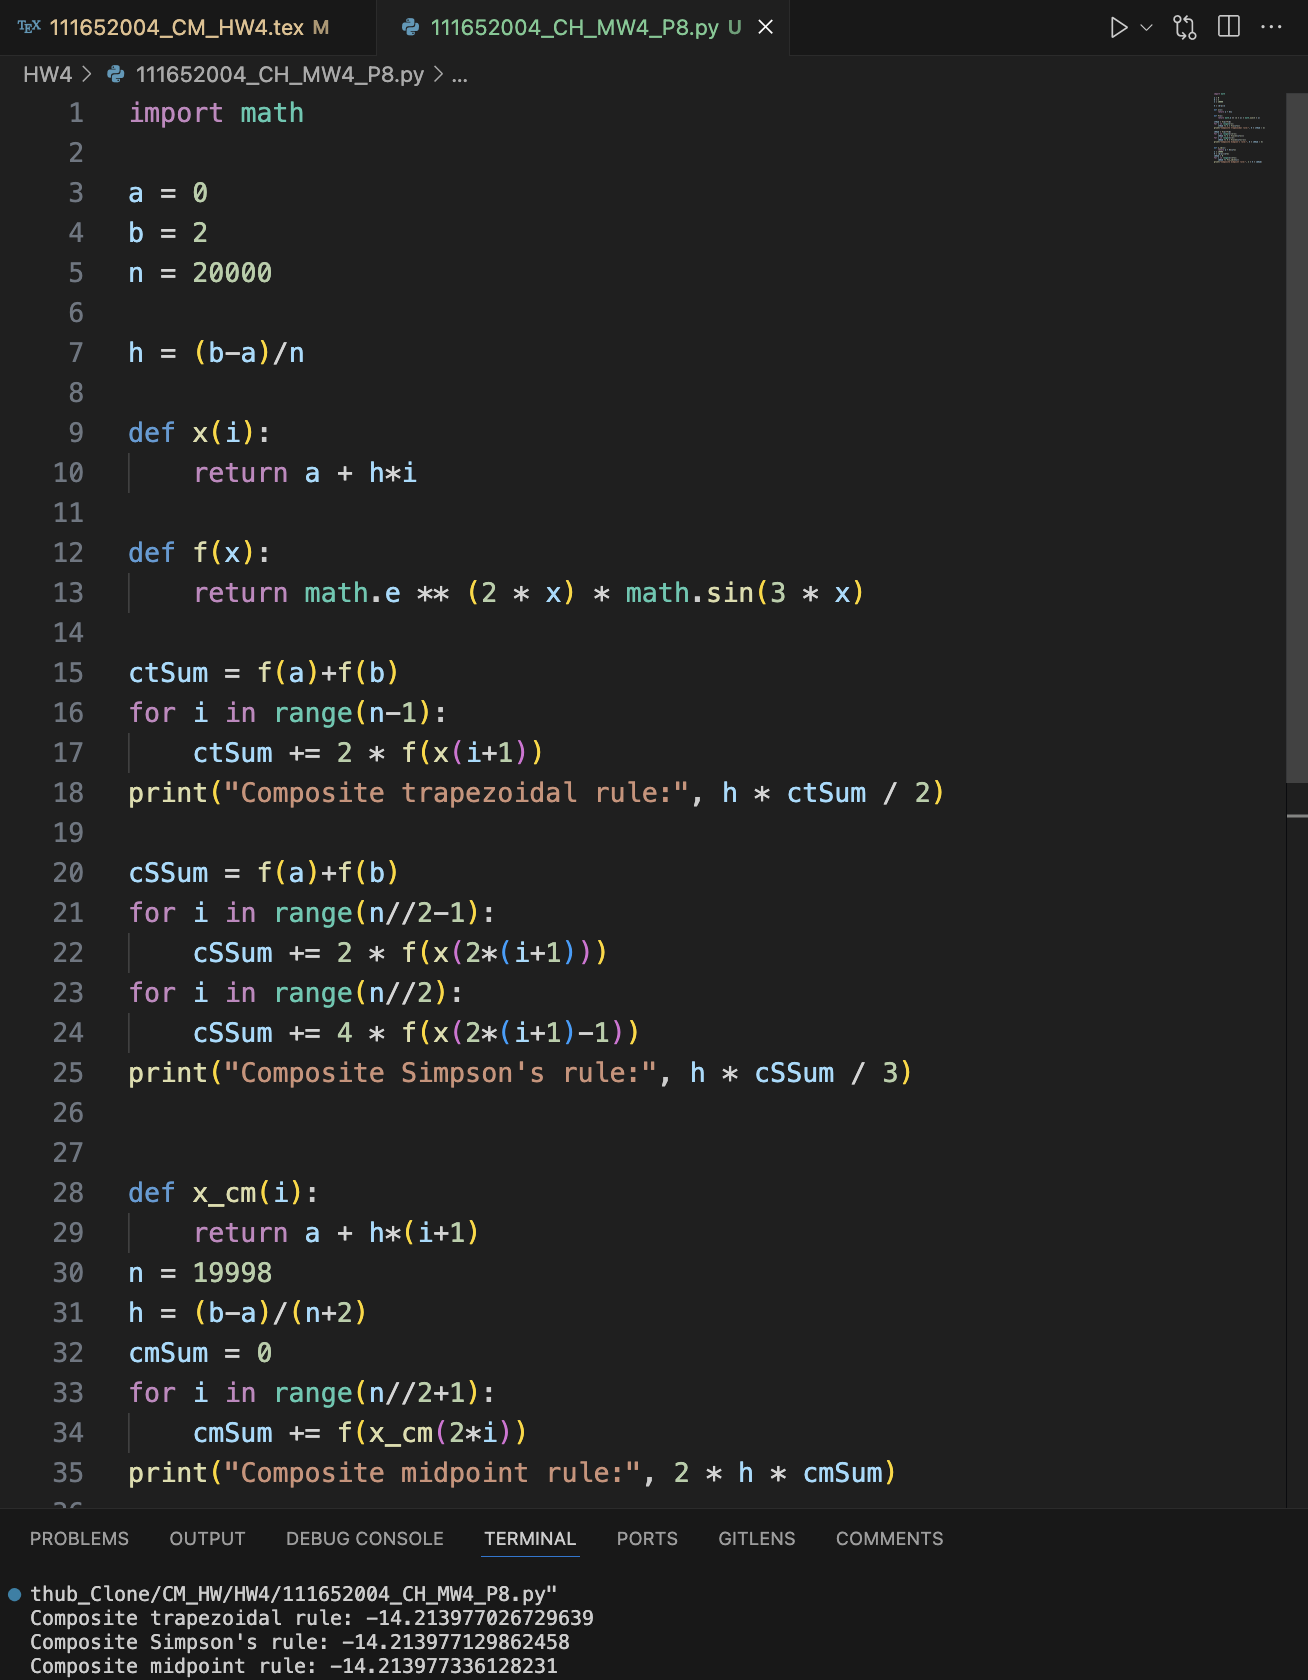
\includegraphics[width=0.8\textwidth]{P8.png}
\end{center}


\newpage
\begin{problem}\label{problem 9} % 4.4 E21
    Determine to within $10^{-6}$ the length of the graph of the ellipse with $4x^2+9y^2=36$.
\end{problem}
\textbf{Solution}. We use composite Simpson's rule to answer. The desired integral is $$2\cdot\int_{0}^{\pi}\sqrt{\left(-3\sin\theta\right)^2+\left(2\cos\theta\right)^2}\ddi\theta.$$ The function $f(x)$ can be re-written as $\displaystyle\sqrt{4+5(\sin\theta)^2}$. Choose $n=1000$, so that the error term \begin{align*}
    \dfrac{\pi-0}{180}\cdot\left(\dfrac{\pi-0}{1000}\right)^4\cdot f^{(4)}(\mu)&\leq\dfrac{\pi-0}{180}\cdot\left(\dfrac{\pi-0}{1000}\right)^4\cdot \sup_{x\in\mathbb{R}}\left|f^{(4)}(x)\right|\\
    &<\dfrac{\pi}{180}\cdot0.01^4\cdot20\\
    &<3.5\times10^{-9}.
\end{align*} By Python and composite Simpson's rule, \begin{align*}
    2\cdot\int_{0}^{\pi}\sqrt{\left(-3\sin\theta\right)^2+\left(2\cos\theta\right)^2}\ddi\theta&\approx2\cdot\dfrac{\pi}{1000}\cdot\dfrac{1}{3}\left[f(0)+2\cdot\sum_{j=1}^{499}f(x_{2j})+4\cdot\sum_{j=1}^{500}f(x_{2j-1})+f(\pi)\right]\\
    &=15.8654393826,
\end{align*} where $x_i=a+hi$. The true value is around $8E\left(-\dfrac{5}{4}\right)=15.8654395893$; thus the absolute error is \begin{align*}
    \left|15.8654393826-15.8654395893\right|&=0.0000002067\\
    &<3\times10^{-7}\\
    &<10^{-6}.
\end{align*} \qed

\begin{center}
    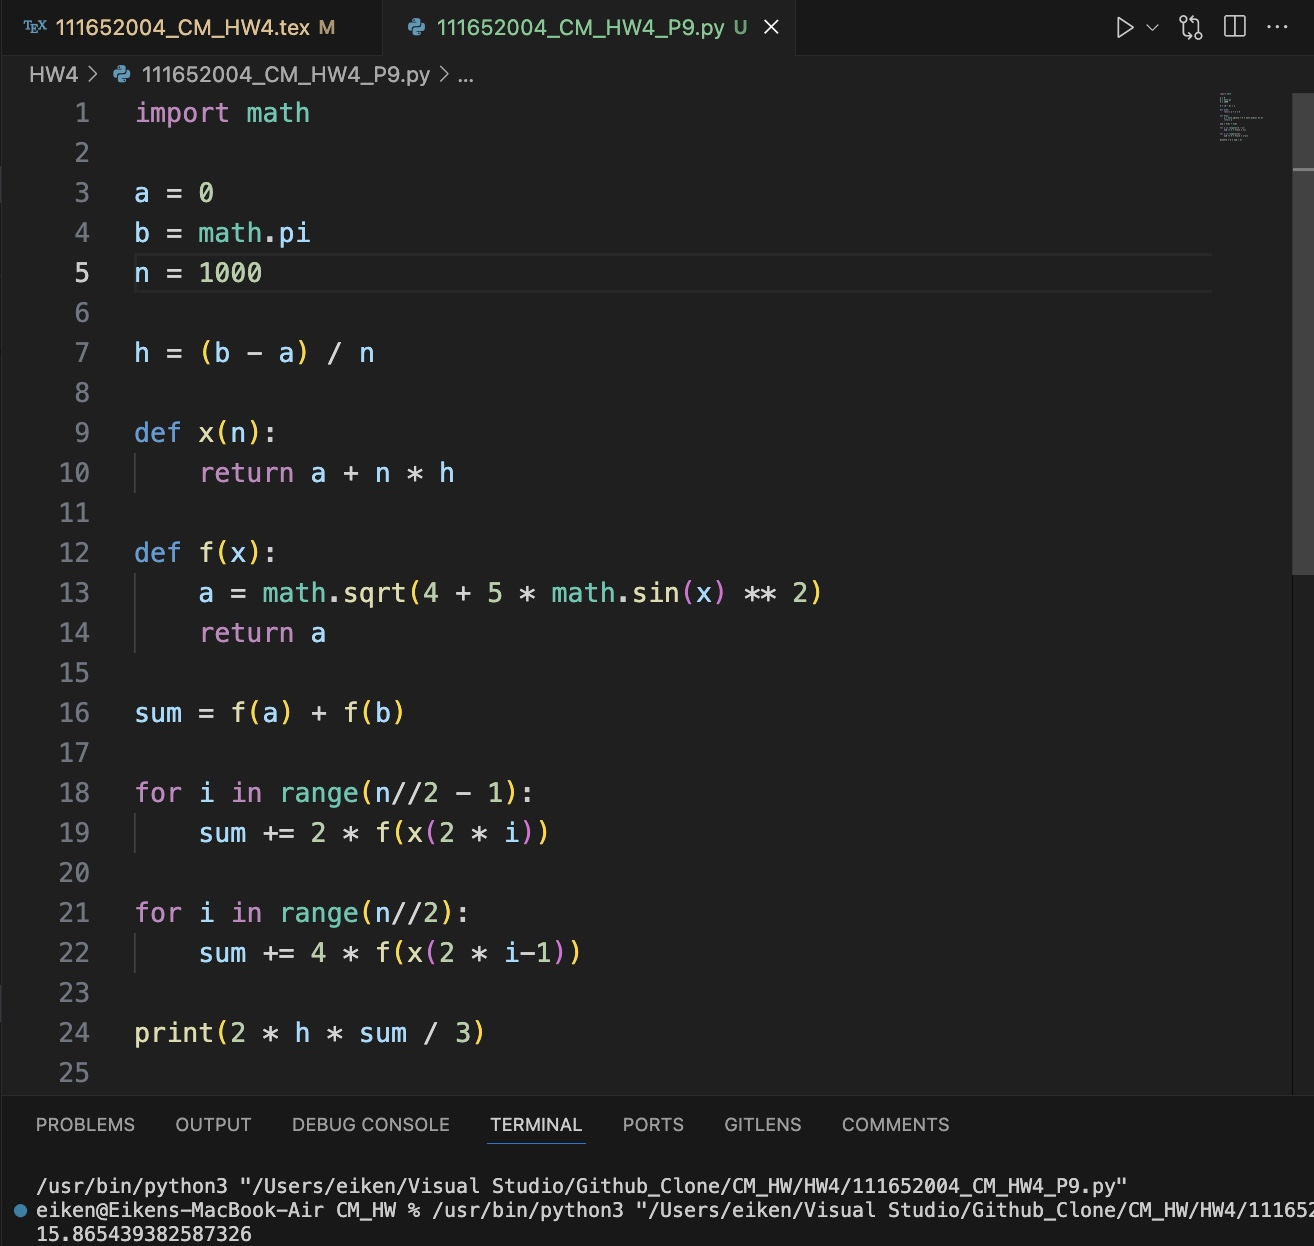
\includegraphics[width=0.8\textwidth]{P9.jpg}
\end{center}


\newpage
\begin{problem}\label{problem 10} % 4.4 E16
    Show that the error $E(f)$ for composite Simpson's rule can be approximated by $$-\dfrac{h^4}{180}\left(f'''(b)-f'''(a)\right).$$ [Hint: $\displaystyle\sum_{j=1}^{n/2}f^{(4)}(\xi_j)(2h)$ is a Riemann sum for $\displaystyle\int_{a}^{b}f^{(4)}(x)\ddi x$.]
\end{problem}
\textbf{Solution}. 


\newpage
\begin{problem}\label{problem 11} % 4.5 E7
    Use the following data to approximate $\displaystyle\int_1^5 f(x)\ddi x$ as accurately as possible.
    \begin{center}
        \begin{tabular}{c|c|c|c|c|c}
            $x$ & $1$ & $2$ & $3$ & $4$ & $5$ \\
            \hline
            $f(x)$ & $2.4142$ & $2.6734$ & $2.8974$ & $3.0976$ & $3.2804$
        \end{tabular}
    \end{center}
\end{problem}
\textbf{Solution}. We use the Romberg extrapolation for higher accuracy. \begin{align*}
    R_{1,1}&=4\cdot\left(2.4142+3.2804\right)=22.7784;\\
    R_{2,1}&=2\cdot\left(2.4142+2.8974+3.2804\right)=17.184;\\
    R_{3,1}&=1\cdot\left(2.4142+2.6734+2.8974+3.0976+3.2804\right)=14.363;\\
    R_{2,2}&=R_{2,1}+\dfrac{1}{4^1-1}\left(R_{2,1}-R_{1,1}\right)\\
    &=15.3192;\\
    R_{3,2}&=R_{3,1}+\dfrac{1}{4^1-1}\left(R_{3,1}-R_{2,1}\right)\\
    &=13.4227;\\
    R_{3,3}&=R_{3,2}+\dfrac{1}{4^2-1}\left(R_{3,2}-R_{2,2}\right)\\
    &=13.2963.
\end{align*} \qed


\newpage
\begin{problem}\label{problem 12} % 4.5 E13
    Show that the approximation obtained from $R_{k,2}$ is the same as that given by the composite Simpson's rule described in Theorem 4.4 with $h=h_k$.
\end{problem}
\textbf{Solution}. 


\newpage
\begin{problem}\label{problem 13} % 4.6 E5
    Use composite Simpson's rule with $n=4, 6, 8,\dots$, until successive approximations to the following integrals agree to within $10^{-6}$. Determine the number of nodes required. Use the adaptive quadrature algorithm to approximate the integral to within $10^{-6}$, and count the number of nodes. Did the adaptive quadrature produce any improvement? \vspace{-1em}
    \begin{multicols}{2}
        \begin{enumerate}
            \item $\displaystyle\int_{0}^{\pi}x\sin(x^2)\ddi x$; and
            \item $\displaystyle\int_{0}^{\pi}x^2\sin x\ddi x$.
        \end{enumerate}
    \end{multicols}
    \vspace{0.1em}
\end{problem}
\textbf{Solution}. 


\newpage
\begin{problem}\label{problem 14} % 4.7 E1
    Approximate the following integral using Gaussian quadrature with $n=2, 3, 4$. Compare your answers with the exact values of the integral. $$\int_{1}^{1.6}\dfrac{2x}{x^2-4}\ddi x.$$
\end{problem}
\textbf{Solution}. We first transform the interval $[1, 1.6]$ to $[-1, 1]$ by using $t=\dfrac{2x-2.6}{0.6}$. Hence the integral becomes $$\int_{-1}^{1}\dfrac{0.6t+2.6}{\left(\frac{0.6t+2.6}{2}\right)^2-4}\cdot\dfrac{0.6}{2}\ddi t=\int_{-1}^{1}\dfrac{6t+26}{3t^2+26t-77}\ddi t.$$ We now deal with the case $n=2$. Using Table 4.12, the approximation is \begin{align*}
    &\quad\ 1\cdot\dfrac{12\cdot 0.57735+26}{(0.57735)^2+26\cdot0.57735-77}+1\cdot\dfrac{12\cdot (-0.57735)+26}{(-0.57735)^2+26\cdot(-0.57735)-77}\\
    &=-0.73072.
\end{align*} We now deal with the case $n=3$. Using Table 4.12, the approximation is \begin{align*}
    &\quad\ 0.55556\cdot\dfrac{12\cdot 0.77460+26}{(0.77460)^2+26\cdot0.77460-77}\\&\quad+0.88889\cdot\dfrac{12\cdot 0+26}{(0)^2+26\cdot0-77}\\&\quad+0.55556\cdot\dfrac{12\cdot (-0.77460)+26}{(-0.77460)^2+26\cdot(-0.77460)-77}\\
    &=-0.73370.
\end{align*} We now deal with the case $n=4$. Using Table 4.12, the approximation is \begin{align*}
    &\quad\ 0.34785\cdot\dfrac{12\cdot 0.86114+26}{(0.86114)^2+26\cdot0.86114-77}\\&\quad+0.65215\cdot\dfrac{12\cdot 0.33998+26}{(0.33998)^2+26\cdot0.33998-77}\\&\quad+0.65215\cdot\dfrac{12\cdot (-0.33998)+26}{(-0.33998)^2+26\cdot(-0.33998)-77}\\&\quad+0.34785\cdot\dfrac{12\cdot (-0.86114)+26}{(-0.86114)^2+26\cdot(-0.86114)-77}\\
    &=-0.73396.
\end{align*} The exact value of the integral is \begin{align*}
    \int_{1}^{1.6}\dfrac{2x}{x^2-4}\ddi x&=\int_{-3}^{-1.44}\dfrac{1}{u}\ddi u\\
    &=\ln(0.48)\\
    &=-0.73397.
\end{align*} The relative errors are $0.0044228$, $0.00022582$, and $0.000012200$, in the order of $n=2$, $n=3$, and $n=4$. The process of calculation is done by Python. \qed

\begin{center}
    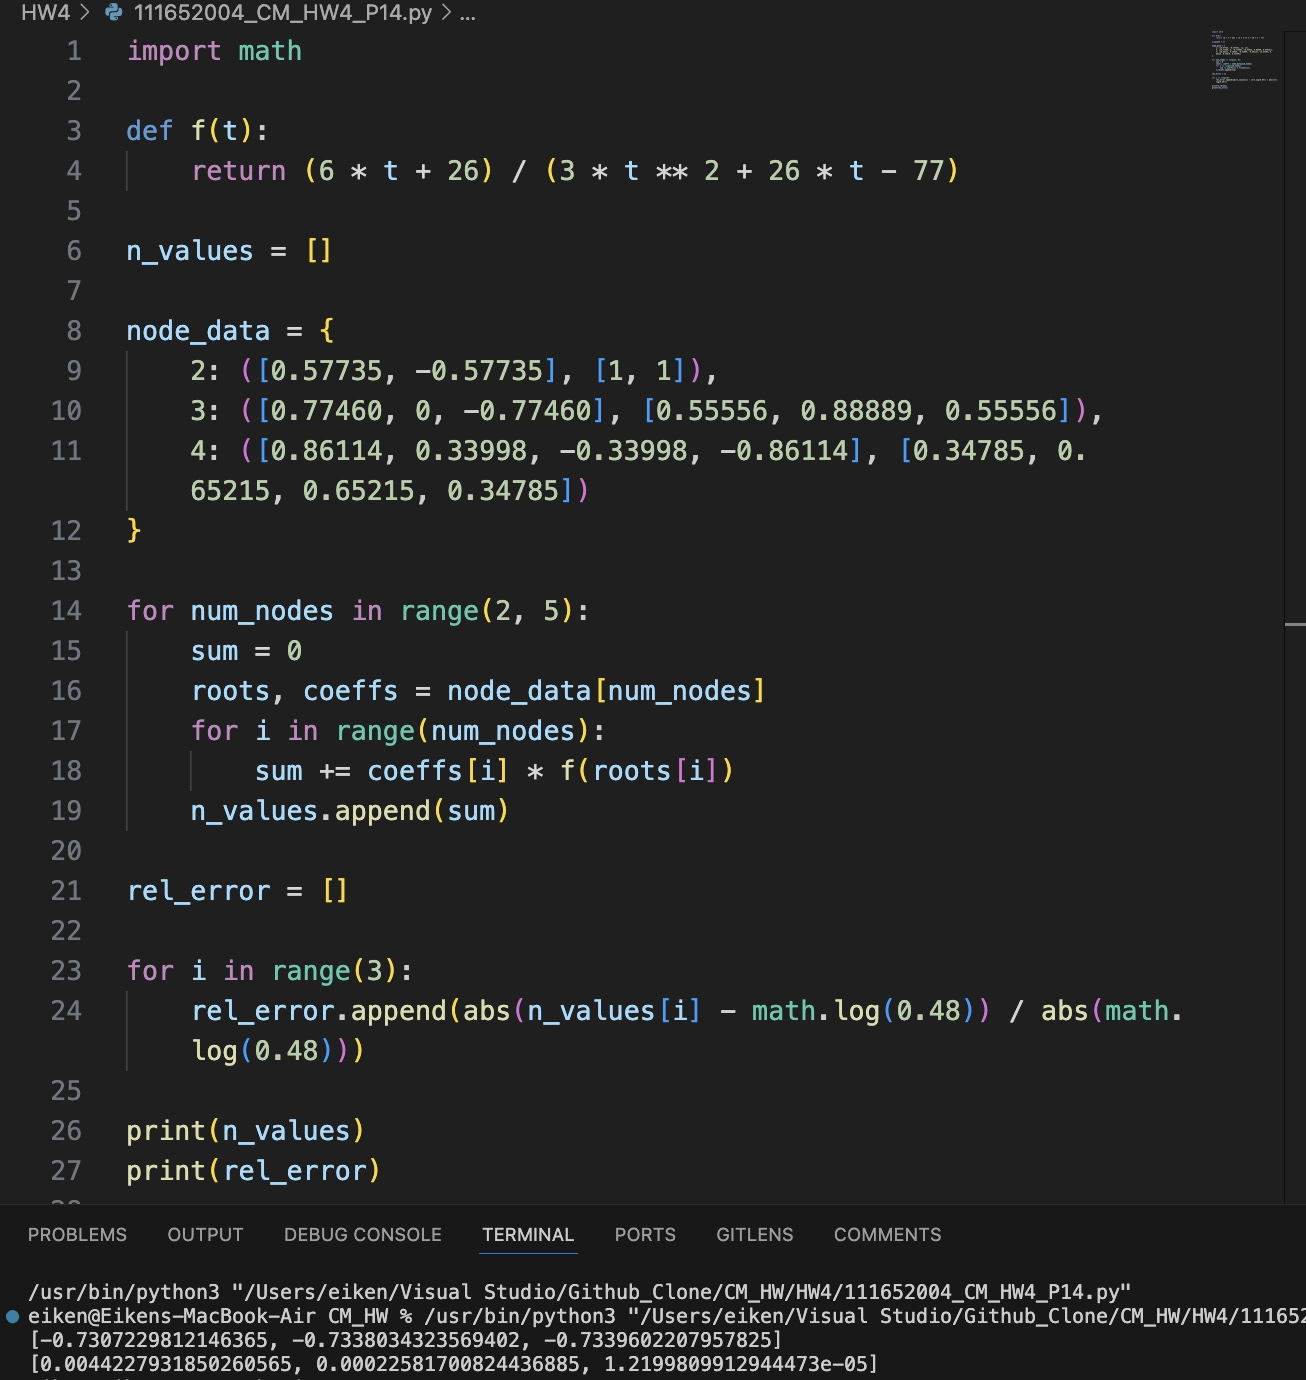
\includegraphics[width=0.8\textwidth]{P14.jpg}
\end{center}


\newpage
\begin{problem}\label{problem 15} % 4.7 E6 Watch the precision
    Determine constants $a$, $b$, $c$, and $d$ that will produce a quadrature formula $$\int_{-1}^{1}f(x)\ddi x=a\cdot f(-1)+b\cdot f(1)+c\cdot f'(-1)+d\cdot f'(1).$$ that has degree of precision $3$.
\end{problem}
\textbf{Solution}. Set $f(x)=P_0(x)=1$. Then $$2=a+b.$$ Set $f(x)=P_1(x)=x$. Then $$0=-a+b+c+d.$$ Set $f(x)=P_2(x)=x^2$. Then $$\dfrac{2}{3}=a+b-2c+2d.$$ Set $f(x)=P_3(x)=x^3$. Then $$0=-a+b+3c+3d.$$ Hence, $(a, b, c, d)=(1, 1, 1/3, -1/3)$. \qed


\newpage
\begin{problem}\label{problem 16} % 4.9 E4
    The improper integral $$\int_{0}^{\infty}f(x)\ddi x$$ cannot be converted into an integral with finite limits using the substitution $t=\dfrac{1}{x}$ because the limit at zero becomes infinite. The problem is resulved by first writing $$\int_{0}^{\infty}f(x)\ddi x=\int_{0}^{1}f(x)\ddi x+\int_{1}^{\infty}f(x)\ddi x.$$ Apply this technique to approximate the following improper integrals to within $10^{-6}$. \vspace{-1em}
    \begin{multicols}{2}
        \begin{enumerate}
            \item $\displaystyle\int_{0}^{\infty}\dfrac{1}{1+x^4}\ddi x$; and
            \item $\displaystyle\int_{0}^{\infty}\dfrac{1}{(1+x^2)^3}\ddi x$.
        \end{enumerate}
    \end{multicols}
    \vspace{0.1em}
\end{problem}
\textbf{Solution}. 


\end{document}